\documentclass{article}
\usepackage[a4paper, hmargin={2.5cm, 2.5cm}, vmargin={2.5cm, 2.5cm}]{geometry}
\usepackage[utf8]{inputenc}
\usepackage[english]{babel}
\usepackage{amsmath,amssymb,graphicx}
\usepackage{cleveref}
\usepackage{hyperref}

\usepackage{mathtools}
\usepackage{fancyhdr}
\usepackage{lastpage}
\usepackage{geometry}
\usepackage{ulem}
\usepackage{gauss}
\usepackage{graphicx}
\usepackage{pdfpages}
\usepackage{hyperref}
\usepackage{cleveref}
\usepackage{wrapfig}
\usepackage{morefloats}
\usepackage{upquote}


%%%%%% COLORS %%%%%%%%

\usepackage{xcolor}
\definecolor{red1}{rgb}{0.7, 0.0, 0.3}
\definecolor{red2}{rgb}{0.5, 0.0, 0.5}
\definecolor{red3}{rgb}{0.3, 0.0, 0.7}

%two definitions of the color grey
\usepackage{color}
\definecolor{listinggray}{gray}{0.9}
%\definecolor{lbcolor}{rgb}{0.9,0.9,0.9}

\usepackage{listings}
\lstset{
	language=,
	literate=
		{æ}{{\ae}}1
		{ø}{{\o}}1
		{å}{{\aa}}1
		{Æ}{{\AE}}1
		{Ø}{{\O}}1
		{Å}{{\AA}}1
		{'}{{'}}1,
	backgroundcolor=\color{listinggray},
	tabsize=3,
	rulecolor=,
	basicstyle=\scriptsize,
	upquote=true,
	aboveskip={1.5\baselineskip},
	columns=fixed,
	showstringspaces=false,
	extendedchars=true,
	breaklines=true,
	prebreak =\raisebox{0ex}[0ex][0ex]{\ensuremath{\hookleftarrow}},
	frame=single,
	showtabs=false,
	showspaces=false,
	showstringspaces=false,
	identifierstyle=\ttfamily,
	keywordstyle=\color[rgb]{0,0,1},
	commentstyle=\color[rgb]{0.133,0.545,0.133},
	stringstyle=\color[rgb]{0.627,0.126,0.941},
}

\lstset{moredelim=[s][\color{gray}]{(*}{*)}}
\lstset{morecomment=[l][\color{gray}]{##}}
\lstset{moredelim=[s][\color{green!50!brown}]{"}{"}}
\lstset{moredelim=[s][\color{green!50!brown}]{'}{'}}
\lstset{moredelim=[s][\color{gray}]{/*}{*/}}

\lstset{literate=
	{0}{{{\color{violet}{0}}}}1
	{1}{{{\color{violet}{1}}}}1
	{2}{{{\color{violet}{2}}}}1
	{3}{{{\color{violet}{3}}}}1
	{4}{{{\color{violet}{4}}}}1
	{5}{{{\color{violet}{5}}}}1
	{6}{{{\color{violet}{6}}}}1
	{7}{{{\color{violet}{7}}}}1
	{8}{{{\color{violet}{8}}}}1
	{9}{{{\color{violet}{9}}}}1
	{?}{{{\color{orange}{?}}}}1
}

\lstset{emph={for, in, if, elif, else, return, def, print}, emphstyle={\color{blue}},,
        emph={[3]std}, emphstyle={[3]\color{green}}}

\lstset{emph={True, False}, emphstyle={\color{violet}},,
        emph={[3]std}, emphstyle={[3]\color{green}}}

%captions on listings
\usepackage[center,font=small,labelfont=bf,textfont=it]{caption}

\title{Insert Assignment Title Here\\02807 Computational Tools for Big Data}
\author{Anonymous authors}
\date{Insert hand in date here}

\setlength\parindent{0pt}		% noindent through whole document
\usepackage[parfill]{parskip}	% extra linebreak on new paragraph

\begin{document}

\maketitle

\section{Exercise 6}
\label{sec:Exercise 6}
\subsection{Exercise 6.1}
\label{sub:Exercise 6.1}

Here you can see we have created a Graph Story account and generated a database:

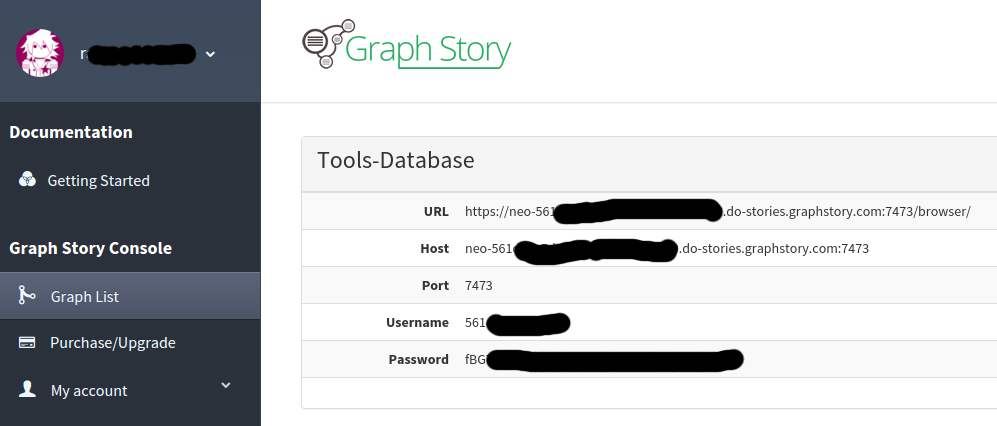
\includegraphics[scale=0.45]{graph_story.png}

Then we removed all data from the database:

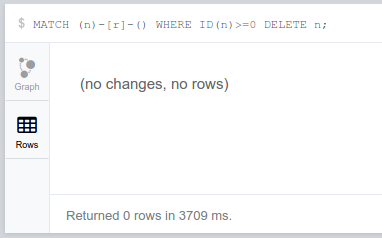
\includegraphics[scale=0.5]{delete_all.png}

Lastly, we loaded all the data into the database, using the given code.
I've chosen to only include the output of the last line of code, which should be
enough proof that we have done them all.

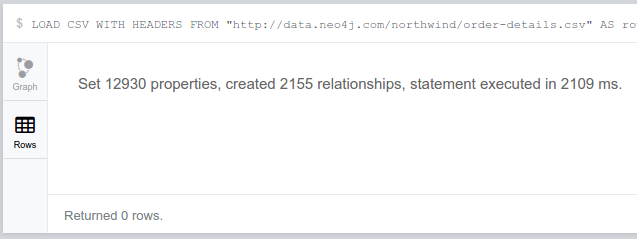
\includegraphics[scale=0.5]{insert_data.png}

\subsection{Exercise 6.2}
\label{sub:Exercise 6.2}

https://neo-561d00e7d6feb-561d00e7dd740.do-stories.graphstory.com:7473/browser/
MATCH (customer {customerID:'ALFKI'})--(orders) RETURN orders

\end{document}
